%% 96_appendix_surface.tex -- Owner group: G5. Rewritten for the camera-ready (2026-10-01).
%% Holds what Section 4.5 summarises: the fitted forms, exponents, coordinate and robustness
%% refits, fit diagnostics, depth optima, figures, and the serving note.
\section{Fitted surface}
\label{app:surface}
The registered analysis fits power laws to the error of each metric, with
$\mathrm{err}_{\mathrm{WER}} = \mathrm{WER}$ and $\mathrm{err}_{\mathrm{SIM}} = 1 -
\text{SIM-o}$. Part~A uses the 15 configurations at $T{=}16$. It compares a fit with
separate width and depth terms, $M_{\mathrm{full}}$:
$\mathrm{err} = E + A\,w^{-\alpha} + B\,d^{-\beta}$, with a fit in the parameter count
alone, $M_N$: $\mathrm{err} = E + C\,N^{-\gamma}$. Part~B uses all \Nsurface\ surface points
and compares the two forms of Eq.~\eqref{eq:models}. In the separable form, steps add their
own power law. In the substitution form, steps enter only through the product $d\,T^{\kappa}$.
\begin{equation}
\label{eq:models}
\begin{aligned}
\text{separable } (M_{\mathrm{sep}})\text{:}\quad &\mathrm{err}_m(w,d,T) = E_m + A_m w^{-\alpha_m} + B_m d^{-\beta_m} + C_m T^{-\tau_m}\\[-1pt]
\text{substitution } (M_{\mathrm{sub}})\text{:}\quad &\mathrm{err}_m(w,d,T) = E_m + A_m w^{-\alpha_m} + B_m \big(d\,T^{\kappa_m}\big)^{-\beta_m}
\end{aligned}
\end{equation}
Table~\ref{tab:exponents} gives the fitted exponents. Figure~\ref{fig:main} shows the
measured step curves behind the surface, and Figure~\ref{fig:diag} the fitted contours.

\begin{table}[!ht]
  \centering
  \caption{Fitted exponents of Part~B ($M_{\mathrm{sep}}$ for $\alpha,\beta,\tau$;
  $M_{\mathrm{sub}}$ for $\kappa$), with run-level bootstrap intervals on $\tau$. The last
  two columns compare forms by $\Delta$AICc \citep{aicc}.}
  \small
  \begin{tabular}{lcccccc}
    \toprule
    Metric & $\alpha$ (width) & $\beta$ (depth) & $\tau$ (steps) & $\kappa$ &
    $\Delta$AICc$_{\mathrm{sub-sep}}$ & $\Delta$AICc$_{\mathrm{full}-N}$\\
    \midrule
    WER   & \NalphaBWER$^{\ddagger}$ & \NbetaBWER & \NtauWER\ \Ntauwerci & \Nkappawer$^{\dagger}$ & $+\NaiccSSWER$ & $\NaiccFNWER$\\
    SIM-o & \NalphaBSIM$^{\ddagger}$ & \NbetaBSIM & \NtauSIM\ \Ntausimci & \Nkappasim$^{\dagger}$ & $+\NaiccSSSIM$ & $\NaiccFNSIM$\\
    \midrule
    \multicolumn{7}{l}{\footnotesize $^{\dagger}$at its bound. $^{\ddagger}$not identified: the
    width amplitude is at its cap.}\\
    \bottomrule
  \end{tabular}
  \label{tab:exponents}
\end{table}

\begin{figure}[!ht]
  \centering
  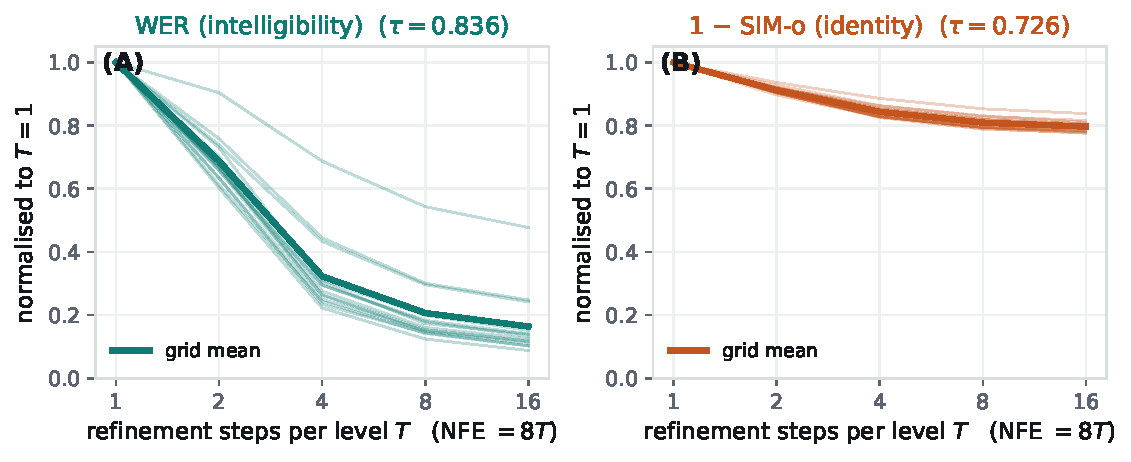
\includegraphics[width=.62\linewidth]{figures/step_curves.pdf}
  \caption{Error against refinement steps for all \Nconfigs\ configurations, each normalised
  to its own $T{=}1$ value; thick lines are grid means. \textbf{(A)}~WER falls by
  \NabsWERgain\ in absolute terms from $T{=}1$ to $16$. \textbf{(B)}~$1-$SIM-o falls by
  \NabsSIMgain\ over the same range. Same models, sampler and items; only $T$ differs.}
  \label{fig:main}
\end{figure}

\paragraph{Coordinate and range.}
The step exponents change when the error is reparameterised (Table~\ref{tab:scope}).
$\Delta\tau$ is negative under \NdtauNflip\ of the maps we tried. It also depends on the
window of $T$ the fit covers: \NdtauRangeEight\ over $T \le 8$, \NdtauRangeSixteen\ over the
declared $T \le 16$, and \NdtauRangeThirtytwo\ and \NdtauRangeSixtyfour\ over $T \le 32$ and
$T \le 64$. The declared interval holds the fit's $1/\mathrm{SE}^{2}$ weights fixed.
Resampling the weights with the runs widens it to \NdtauHonestci.

\begin{table}[!ht]
  \centering
  \caption{The same \Nsurface\ measurements refitted after a monotone change of both errors.
  The last column is the share ratio of Table~\ref{tab:gapclosed}; --- marks rows where it was
  not computed.}
  \label{tab:scope}
  \small
  % GENERATED by src/paper_v14.py
\begin{tabular}{lcccc}
  \toprule
  error coordinate & $\tau_{\mathrm{WER}}$ & $\tau_{\mathrm{SIM}}$ & $\Delta\tau$ & gap-closed ratio \\
  \midrule
    identity \emph{(pre-registered)} & 0.8362 & 0.7260 & +0.1102 & 1.86$\times$ \\
    log(1+err) & 0.6665 & 0.6913 & -0.0248 & 1.85$\times$ \\
    sqrt(err) & 0.4325 & 0.6842 & -0.2517 & 1.68$\times$ \\
    err capped at 1 & 0.7093 & 0.7260 & -0.0167 & n/a \\
    err squared & 1.5613 & 0.8122 & +0.7491 & 1.82$\times$ \\
    affine 3+2*err (v1.0 check) & 0.7600 & 0.7249 & +0.0351 & n/a \\
  \bottomrule
\end{tabular}

\end{table}

\paragraph{Other refits of $\Delta\tau$.}
$\Delta\tau$ stays positive when one factor of the fit changes (Table~\ref{tab:robust}): a
fourth parameter budget, $3\times$ training compute, a different ASR, or amplitudes freed on
a log scale. These rows test the sign of $\Delta\tau$ only. The log-amplitude refit does not
identify $\alpha$ (see below). The released \texttt{fits.json} also holds an unweighted
refit, which gives a positive $\Delta\tau$.

\begin{table}[!ht]
  \centering\small
  \caption{$\Delta\tau$ when one factor of the fit changes. Each row refits the surface with
  that factor changed.}
  \begin{tabular}{llcc}
    \toprule
    variation & what changes & $\Delta\tau$ & 95\% CI \\
    \midrule
    none (\Nsurface\ points, \Nruns\ runs) & --- & \Ndtau & \Ndtauci \\
    fourth budget, \NmaxNfour\,M & 10 further runs & \Ndtaufour & \Ndtaufourci \\
    $3\times$ training compute & 3 configs at 90k steps & \Ndtaunineok & \Ndtaunineokci \\
    ASR swapped & Whisper-medium.en \citep{whisper} & \Ndtauasr & \NdtauAsrCI \\
    amplitudes on a log scale & $\log A, \log B, \log C$ free & \Ndtaulogamp & \NdtauLogCI \\
    \bottomrule
  \end{tabular}
  \label{tab:robust}
\end{table}

\paragraph{Fit diagnostics.}
\label{app:diag}
Each form is fitted by weighted non-linear least squares from 32 starting points
(\texttt{src/fit.py}), and the bootstrap refits it on each resample of runs. Amplitudes are bounded to $[0, \NcrsAmpCap]$, exponents to at most \NcrsExpCap, $\kappa$ to
$[-\NcrsKappaBound, \NcrsKappaBound]$ and $E$ to $[0, 1]$. The width amplitude $A$ is at its
cap in all four declared fits: \NcrsApartAWER\ and \NcrsApartASIM\ in Part~A, and
\NcrsApartBWER\ and \NcrsApartBSIM\ in Part~B, for WER and SIM-o. Across all committed fits it is at the cap in
\NcrsAmpFitsAtCap\ of \NcrsAmpFits\ and at zero in \NcrsAmpFitsAtZero. In the bootstrap, $A$
is at the cap in \NcrsAmpBootFullWER\ (Part~A) and \NcrsAmpBootSepWER\ (Part~B) of
\NcrsAmpBootN\ WER replicates, and in every SIM-o replicate. So only the product
$A\,w^{-\alpha}$ is constrained, and $\alpha$ is not identified. Freeing the amplitudes on a
log scale does not help: $\alpha_{\mathrm{WER}}$ then sits at its upper bound
(\NcrsLogampAlphaWER, CI \NcrsLogampAlphaWERci). $\kappa$ is at its upper bound in
\NcrsSubFitsAtBound\ of \NcrsSubFits\ committed substitution fits, and in
\NcrsKappaBootWER\ (WER) and \NcrsKappaBootSIM\ (SIM-o) of \NcrsNboot\ replicates. $E$
reaches zero for WER under $M_{\mathrm{sep}}$. The depth amplitude $B$ is interior in the
declared fits, so $\beta$ is identified: $\beta_{\mathrm{WER}} = \NbetaBWER$ and
$\beta_{\mathrm{SIM}} = \NbetaBSIM$. Points are weighted by $1/\mathrm{SE}^{2}$, with SE taken
over seeds and floored at a quarter of the pooled seed standard deviation;
\texttt{fits.json} records how many points hit the floor. In all three budgets, the spread of
configuration means at $T{=}16$ passes the registered power criterion for both metrics.

\begin{figure}[!ht]
  \centering
  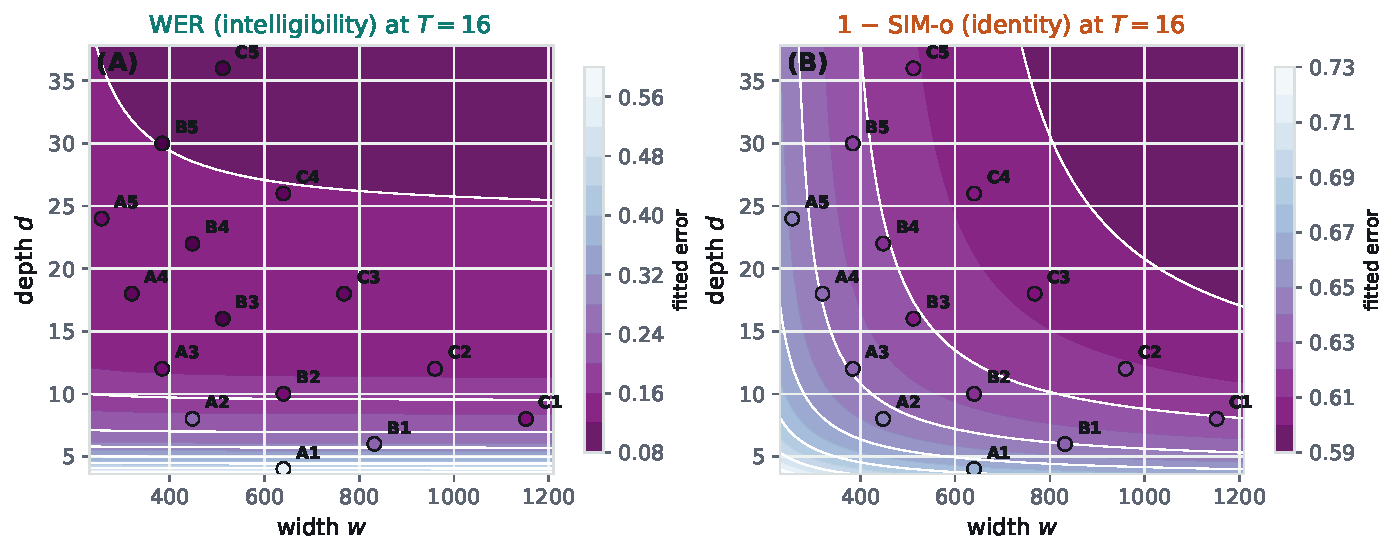
\includegraphics[width=.8\linewidth]{figures/aniso_contours_T16.pdf}\\[4pt]
  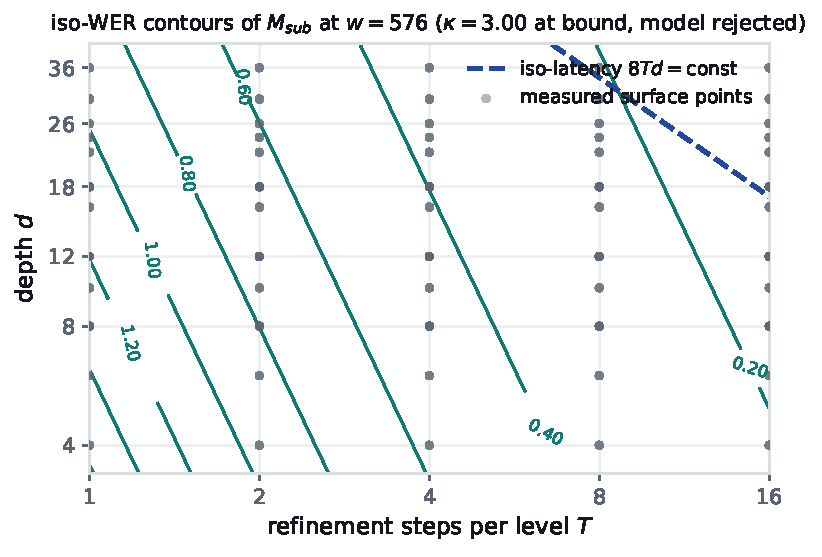
\includegraphics[width=.5\linewidth]{figures/substitution_plane.pdf}
  \caption{\emph{Top:} fitted error contours of $M_{\mathrm{full}}$ in $(w, d)$ at $T{=}16$,
  with the 15 configurations. The width amplitude is at its cap, so the contours' width
  direction is not identified. \emph{Bottom:} iso-WER contours of $M_{\mathrm{sub}}$ at
  $w{=}576$ over the measured $(T, d)$ points, with $\kappa$ at its bound; the dashed line is
  one iso-latency curve ($8Td$ constant).}
  \label{fig:diag}
\end{figure}

\paragraph{Depth optima.}
Table~\ref{tab:dstar} gives the best depth per budget at $T{=}16$. For WER it is the deepest
shape in budgets B and C, so those two values are lower bounds on the WER-optimal depth. No
margin exceeds two standard errors of the difference between two configuration means. Over all
five values of $T$ in the grid, the WER-best depth is the deepest shape in
\NcrsDeepCellsWER\ of the \NcrsDepthCells\ (budget, $T$) cells of budgets A to C, and the
SIM-o-best depth in \NcrsDeepCellsSIM.

\begin{table}[!ht]
  \centering\small
  \caption{Best depth per budget at $T{=}16$, from configuration means. Margin: WER points
  between the best and the runner-up shape; SE: standard error of a configuration mean;
  SE$_{\Delta}$: of the difference of two means ($\sqrt{2}\,$SE). Where the WER-best $d$
  equals the deepest $d$, it is a lower bound on the optimum.}
  \begin{tabular}{lcccccc}
    \toprule
    budget & deepest $d$ & WER-best $d$ & margin & SE & SE$_{\Delta}$ & SIM-o-best $d$ \\
    \midrule
    A & \NcrsDeepestA & \NcrsDstarAWER & \NcrsDstarMarginAWER & \NcrsDstarSEAWER & \NcrsDstarSEdiffAWER & \NcrsDstarASIM \\
    B & \NcrsDeepestB & \NcrsDstarBWER & \NcrsDstarMarginBWER & \NcrsDstarSEBWER & \NcrsDstarSEdiffBWER & \NcrsDstarBSIM \\
    C & \NcrsDeepestC & \NcrsDstarCWER & \NcrsDstarMarginCWER & \NcrsDstarSECWER & \NcrsDstarSEdiffCWER & \NcrsDstarCSIM \\
    D (\NmaxNfour\,M) & \NcrsDeepestD & \NcrsDstarDWER & \NcrsDstarMarginDWER & \NcrsDstarSEDWER & \NcrsDstarSEdiffDWER & \NcrsDstarDSIM \\
    \bottomrule
  \end{tabular}
  \label{tab:dstar}
\end{table}

\paragraph{Extrapolation.}
Figure~\ref{fig:extrap} shows the registered extrapolation test (H-D4). For WER, the mean
absolute percentage error is \NmapeWER\% for $M_{\mathrm{full}}$ and \NmapeNWER\% for $M_N$,
both above the registered 15\% limit. For SIM-o it is \NmapeSIM\% against \NmapeNSIM\%, so
the fitted form does no better than the $N$-only model.

\begin{figure}[!ht]
  \centering
  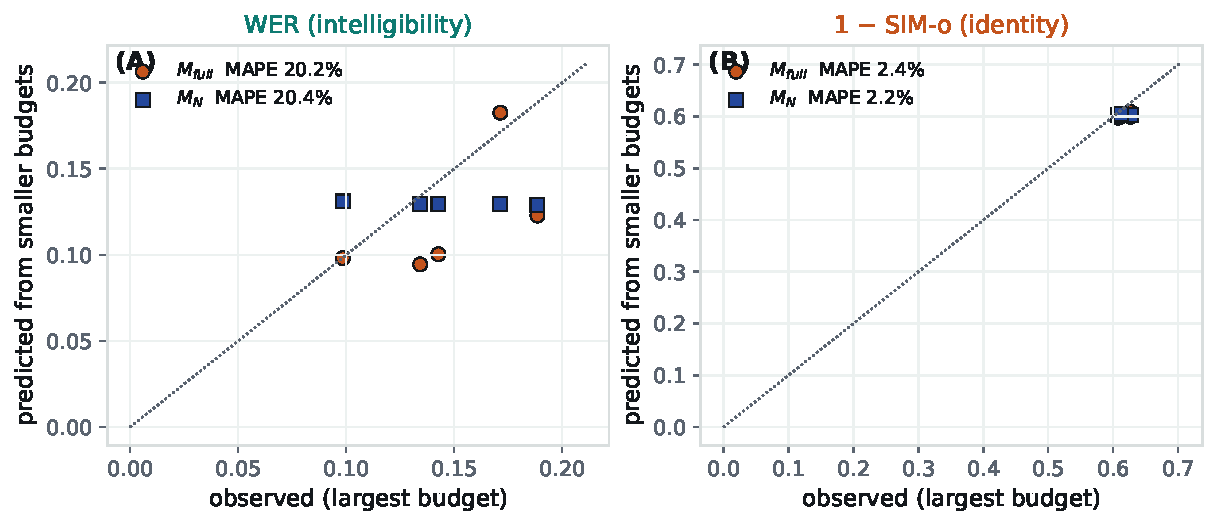
\includegraphics[width=.75\linewidth]{figures/extrapolation.pdf}
  \caption{Extrapolation test (H-D4): $M_{\mathrm{full}}$ and $M_N$ fitted on the two smaller
  budgets at $T{=}16$ and used to predict the largest. The dotted line marks a perfect
  prediction.}
  \label{fig:extrap}
\end{figure}

\paragraph{Serving latency.}
At batch 1, per-layer latency is flat in width on our device: \Nclayerrange\,ms per layer
for $w$ from 256 to 1152. Serial latency is then $8\,T\,d\,c_{\mathrm{layer}}$, so at fixed
parameter count a latency budget constrains only the product $T\,d$. The registered rule for
splitting that product, depth before steps (H-E2), had to agree with the measured best split
at 80\% or more of the tested latency budgets, and it did not. The latency analysis stops at
$T{=}16$, so we do not read this failure as evidence for the reverse rule.
